% Author: Patrik Skaloš (xskalo01)

\documentclass{article}
\usepackage[slovak]{babel}
\usepackage[a4paper]{geometry}
\usepackage{graphicx}
\usepackage{float}
\usepackage{amssymb}

\title{ISS projekt 2021/2022 v jazyku Python}
\author{Patrik Skaloš (xskalo01)}

\begin{document}
  \maketitle


  \section{Základy}
  Počet vzorkov: 32666 vzorkov \\
  Dĺžka signálu [s]:  2.041625 s \\
  Minimálna hodnota: -5418 \\
  Maximálna hodnota: 5299 \\
  \begin{figure}[H]
    \includegraphics[width=\textwidth]{src/input_signal.eps}
    \caption{Vizualizácia vstupného signálu}
  \end{figure}

  \newpage


  \section{Predspracovanie a rámce}
  Počet rámcov: 62
  \begin{figure}[H]
    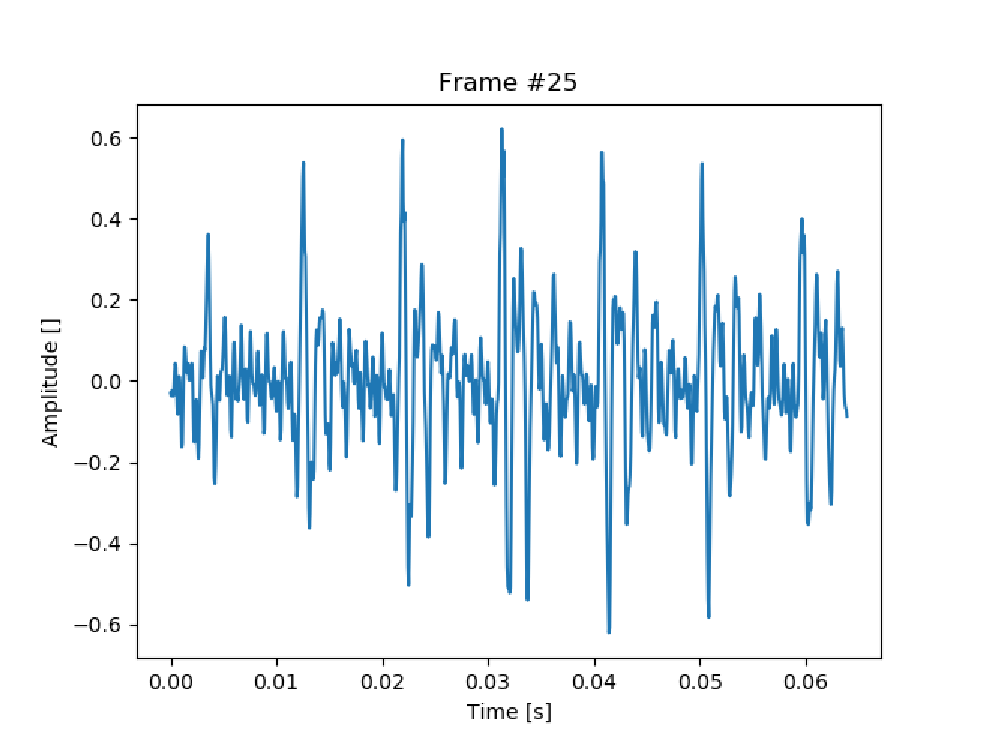
\includegraphics[width=\textwidth]{src/frame25.eps}
    \caption{Vizualizácia rámcu 25}
  \end{figure}


  \section{DFT}

  Vzorec, podľa ktorej som implementoval funkciu DFT: \\
  \verb|X[k] = sum from 0 to N-1 of (x[n] * e^(-jkn2pi / N))| \\

  \noindent
  Kód implementujúci DFT:
  \begin{verbatim}
    coeffs = []
    e = np.exp(-1j * 2 * np.pi / N)
    for k in range(0, N // 2):
        coeffs.append(sum(x * [e ** (k * n) for n in range(N)]))
    return coeffs
  \end{verbatim}

  \newpage
  Výsledok DFT a FFT: \\
  \begin{figure}[h]
    \centering
    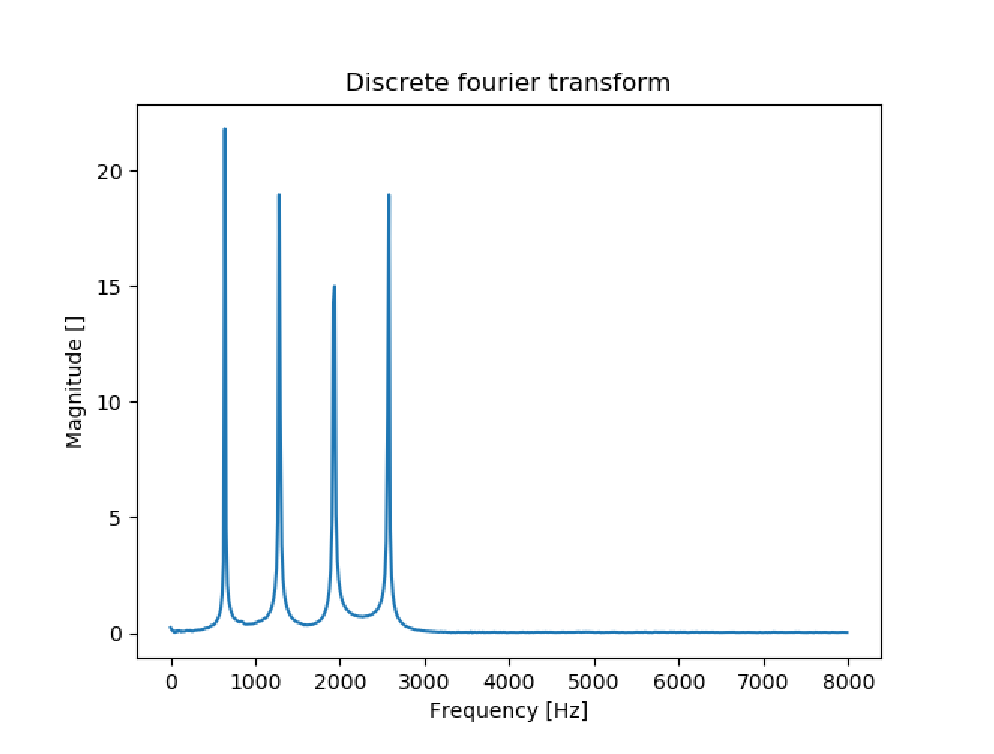
\includegraphics[width=0.62\textwidth]{src/dft.eps}
    \caption{Výsledok DFT implementovanej mnou}
  \end{figure}
  \begin{figure}[h]
    \centering
    \includegraphics[width=0.62\textwidth]{src/fft.eps}
    \caption{Výsledok FFT z knižnice numpy}
  \end{figure}
  \\
  Výsledky oboch transformácií nie sú úplne rovnaké, ale na naše účely 
  dostatočne podobné.


  \section{Spektrogram}

  \begin{figure}[H]
    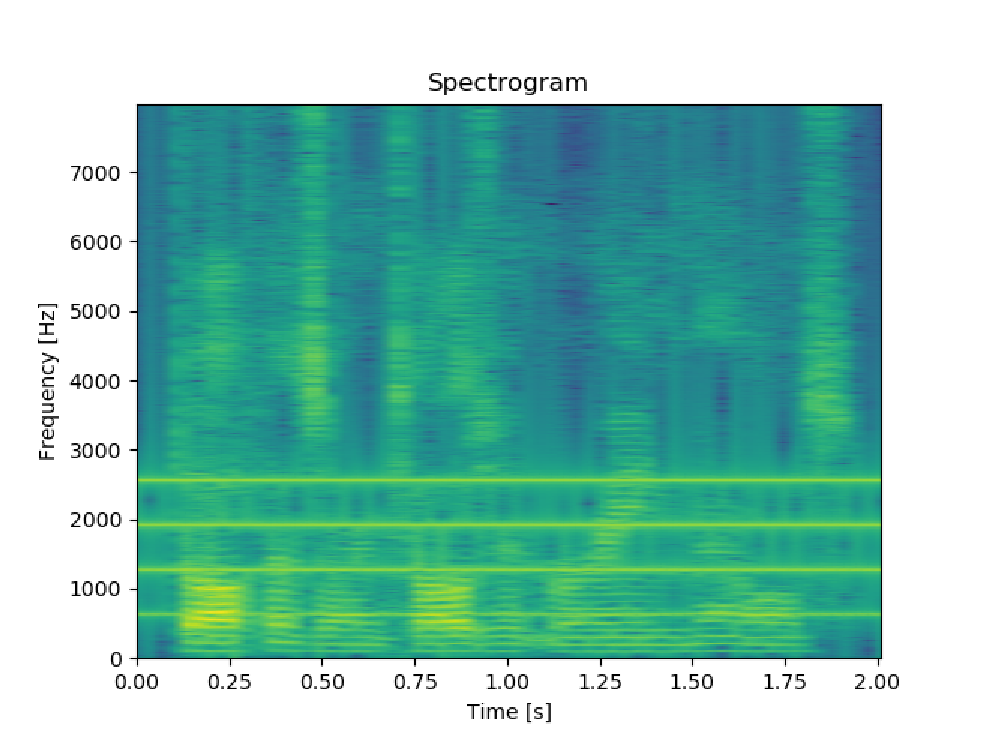
\includegraphics[width=\textwidth]{src/spectrogram.eps}
    \caption{Spektrogram vstupného signálu}
  \end{figure}


  \section{Určenie rušivých frekvencií}
  Približné hodnoty rušivých frekvencií: \\
  \verb|[640, 1281, 1937, 2578]| \\

  \noindent
  Frekvencie $f_2$, $f_3$ a $f_4$ sú násobkami $f_1$: \\
  $f_1 = 640Hz$ \\
  $f_2 = 1281Hz \approxeq 1280Hz = f_1 \times 2 = 640Hz \times 2$ \\
  $f_3 = 1937Hz \approxeq 1920Hz = f_1 \times 3 = 640Hz \times 3$ \\
  $f_4 = 2578Hz \approxeq 2560Hz = f_1 \times 4 = 640Hz \times 4$


  \section{Generovanie signálu}

  \begin{figure}[H]
    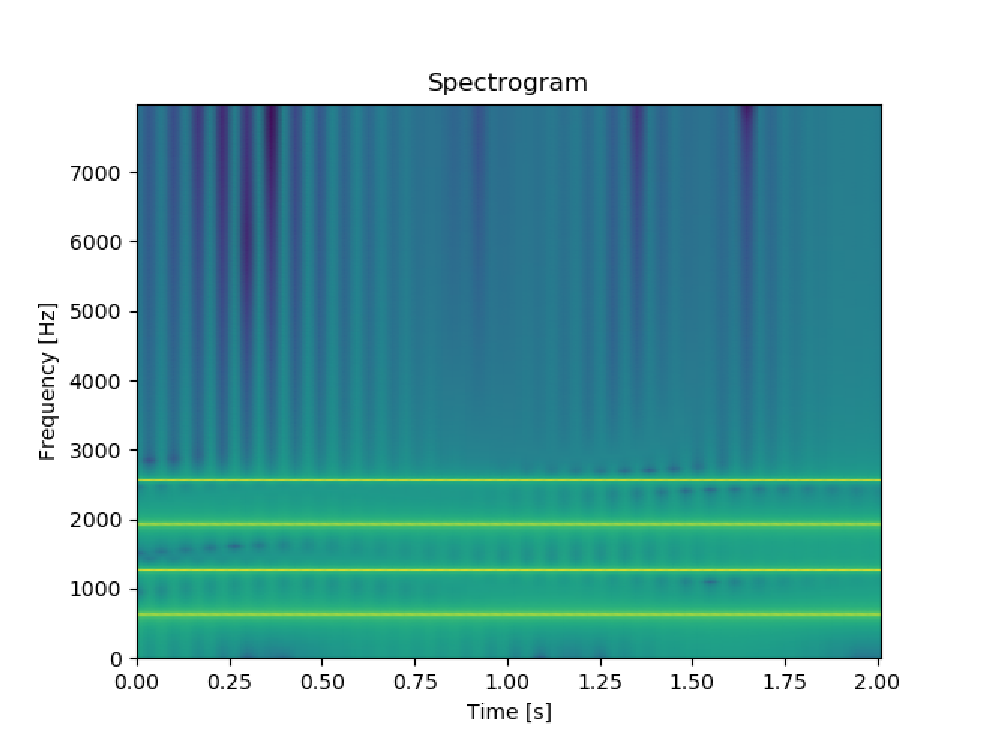
\includegraphics[width=\textwidth]{src/spectrogram_cos.eps}
    \caption{Spektrogram rušivého signálu}
  \end{figure}


  \section{Čistiaci filter}
  Na filtrovanie som navrhol štyri pásmové zádrže s koeficientmi: \\
  Pre frekvenciu $f_1$ \\
  \begin{verbatim}
    [0.95160418 -1.84344975  0.95160418  1.         -1.8992227   0.9645675 ] 
    [1.         -1.93720224  1.          1.         -1.90820475  0.96648921]
    [1.         -1.93720224  1.          1.         -1.91302077  0.98460339]
    [1.         -1.93720224  1.          1.         -1.93227324  0.98655595]
  \end{verbatim}
  Pre frekvenciu $f_2$ \\
  \begin{verbatim}
    [0.95078858 -1.66603958  0.95078858  1.         -1.7140524   0.96447967]
    [1.         -1.75227134  1.          1.         -1.72887515  0.96540549]
    [1.         -1.75227134  1.          1.         -1.72137266  0.98486009]
    [1.         -1.75227134  1.          1.         -1.7563684   0.9858039 ]
  \end{verbatim}
  Pre frekvenciu $f_3$ \\
  \begin{verbatim}
    [0.95046273 -1.37702717  0.95046273  1.         -1.41287617  0.96443744]
    [1.         -1.4487966   1.          1.         -1.43343204  0.96497972]
    [1.         -1.4487966   1.          1.         -1.41285197  0.98495647]
    [1.         -1.4487966   1.          1.         -1.46242588  0.98550968]
  \end{verbatim}
  Pre frekvenciu $f_4$ \\
  \begin{verbatim}
    [0.95028744 -1.00703395  0.95028744  1.         -1.02836091  0.96442036]
    [1.         -1.0597151   1.          1.         -1.05342296  0.96474506]
    [1.         -1.0597151   1.          1.         -1.02108379  0.9850142 ]
    [1.         -1.0597151   1.          1.         -1.08196273  0.98534553]
  \end{verbatim}

  % Inšpiroval som sa zadaním a použil 30Hz šírku záverného pásma, 50Hz šírku 
  % priepustného pásma 

  \begin{figure}[H]
    \includegraphics[width=\textwidth]{src/impulse.eps}
    \caption{Impulzné odozvy filtrov}
  \end{figure}


  \newpage
  \section{Nulové body a póly}

  Nuly:
  \begin{verbatim}
    0.7243983+0.68938168j 0.7243983+0.68938168j 0.7243983+0.68938168j
    0.7243983+0.68938168j 0.7243983-0.68938168j 0.7243983-0.68938168j
    0.7243983-0.68938168j 0.7243983-0.68938168j
  \end{verbatim}
  Póly:
  \begin{verbatim}
    0.73121294+0.67144421j 0.71671602+0.67178708j 0.71671602-0.67178708j
    0.73121294-0.67144421j 0.70642598-0.69707876j 0.70643808-0.68218962j
    0.70643808+0.68218962j 0.70642598+0.69707876j
  \end{verbatim}

  \begin{figure}[H]
    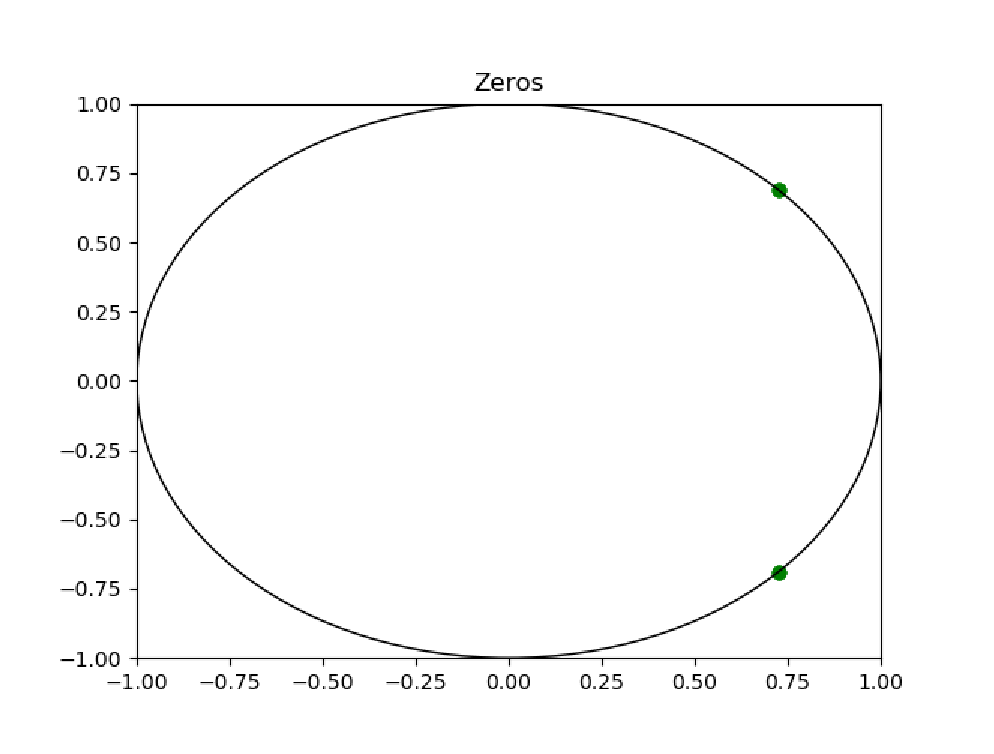
\includegraphics[width=\textwidth]{src/zeros.eps}
    \caption{Nuly}
  \end{figure}
  \begin{figure}[H]
    \centering
    \includegraphics[width=0.8\textwidth]{src/poles.eps}
    \caption{Póly}
  \end{figure}


  \section{Frekvenčná charakteristika}

  \begin{figure}[H]
    \centering
    \includegraphics[width=0.9\textwidth]{src/frequency_responses.eps}
    \caption{Frekvenčné charakteristiky filtrov}
  \end{figure}


  \newpage
  \section{Filtrácia}

  Vstupný signál som filtroval všetkými štyroma filtrami po jednom.

  \begin{figure}[H]
    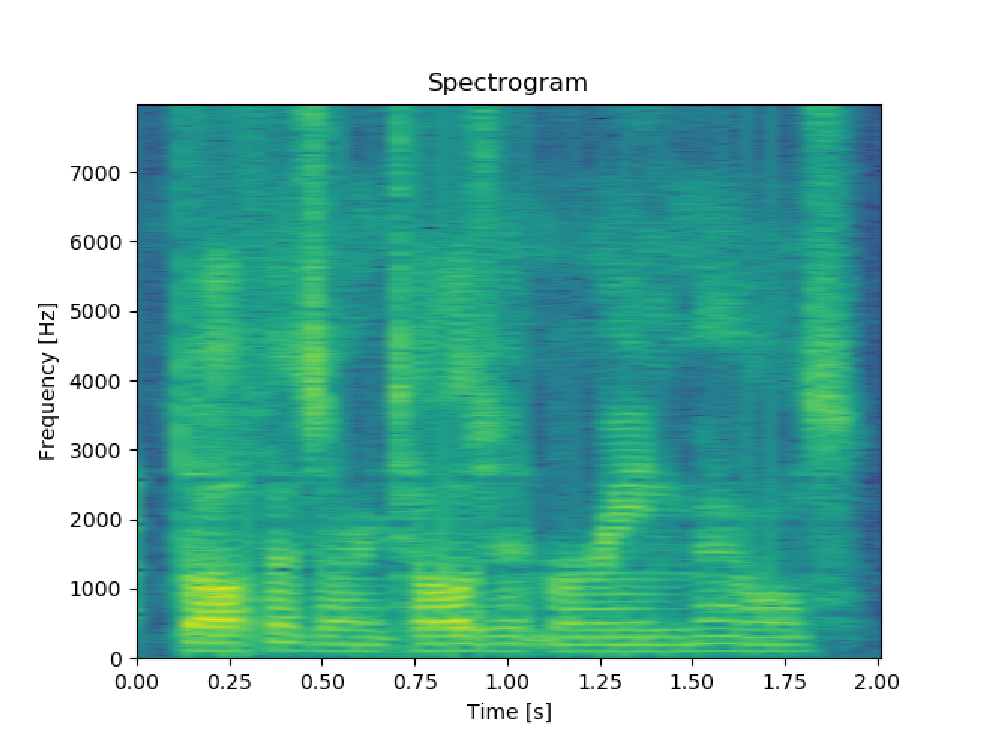
\includegraphics[width=\textwidth]{src/spectrogram_output.eps}
    \caption{Spektrogram výstupného (filtrovaného) signálu}
  \end{figure}

  \section{Záver}

  Pohľadom na spektrogram a posluchom výstupnej nahrávky usudzujem, že sa 
  rušivé frekvencie úspešne podarilo odfiltrovať.


\end{document}
